%\documentclass[iop]{emulateapj}
%\documentclass[12pt, preprint]{emulateapj}
\documentclass[12pt, onecolumn]{emulateapj}

\usepackage{tikz}
\usetikzlibrary{shapes.geometric, arrows}
\usetikzlibrary{fit}

\tikzstyle{hyper} = [circle, text centered, draw=black]%, fill=blue!30]
\tikzstyle{param} = [circle, text centered, draw=black]%, fill=green!30]
\tikzstyle{data} = [circle, text centered, draw=black, line width=2pt]%, fill=red!30]
%\tikzstyle{hyper} = [trapezium, trapezium left angle=70, trapezium right angle=110, minimum width=1cm, minimum height=0.5cm, text centered, draw=black, fill=green!30]
%\tikzstyle{param} = [rectangle, minimum width=1cm, minimum height=0.5cm, text centered, draw=black, fill=green!30]
%\tikzstyle{data} = [diamond, minimum width=1cm, minimum height=1cm, text centered, draw=black, fill=red!30]
%\tikzstyle{eqn} = [rectangle, minimum width=1cm, minimum height=0.5cm, text centered, draw=black]%, fill=green!30]
%\tikzstyle{latent} = [diamond, minimum width=1cm, minimum height=0.5cm, text centered, draw=black]%, fill=green!30]
\tikzstyle{arrow} = [thick,->,>=stealth]

\newcommand{\myemail}{aimalz@nyu.edu}
\newcommand{\textul}{\underline}

\shorttitle{Probabilistic Redshift Distribution}
\shortauthors{Malz}

\begin{document}

\title{Probabilistic Redshift Distribution: Minimal Approach}

\author{A.I. Malz\altaffilmark{1}}
\altaffiltext{1}{CCPP}
\email{aimalz@nyu.edu}

\begin{abstract}
Upcoming galaxy surveys aim to produce posterior probability distribution functions on photometric redshift (zPDFs) for each galaxy observed, but no one has yet clearly presented a mathematically valid method for how to use zPDFs to do inference on the physical parameters relevant to galaxy evolution, large-scale structure, and cosmology.  By considering a generative model for zPDFs, this paper presents a fully consistent technique for calculating the redshift density function $n(z)$ from a set of zPDFs as an example of how such data products should be used.  
\end{abstract}

\keywords{photo-z}

\section{Introduction}

The era of precision cosmology has been enabled by photometric estimation of redshifts previously determined by time- and resource-intensive spectroscopic confirmation.  However, photometric redshifts (photo-zs) are susceptible to a number of errors, particularly their inherent noisiness due to the coarseness of photometric filters and catastrophic errors in which galaxies of one type at one redshift are mistaken for galaxies of another type at a different redshift.  In addition to these limitations in accuracy, there is also the matter of precision.  Photo-zs are often reported with error bars derived without inclusion of all systematic errors.

An alternative to point estimates of photo-zs is redshift probability distribution function (zPDF) estimation.  An extension of \citet{ben00} that produces full posteriors (as opposed to a selection of local maxima) from a template library of galaxy spectral energy distributions (SEDs) has been mentioned in the litertature \citep{lop14}, but a formal presentation has not yet been published.  zPDFs have also been obtained by a variety of trustworthy data-driven approaches in the literature: $k$-nearest neighbor algorithms with \citep{bal08} and without \citep{she11} inclusion of photometric measurement errors, neural networks \citep{bon13}, self-organizing maps \citep{car14}, prediction tree and random forest classification techniques \citep{car13}.  Redshift posterior distributions have been produced by completed surveys \citep{she11} and will be produced by upcoming surveys \citep{abe09}.

However, zPDFs have seldom been used in inference of physical parameters.  Furthermore, no implementation of inference from zPDFs has been backed by a mathematically consistent methodology.  The goal of this paper is to present and validate a method for the use of zPDFs in inference.  For simplicity, we shall consider only one-point statistics relevant to cosmology; future work will focus on higher-order statistics of redshift.  For ease of comparison with previous work, we choose to investigate the redshift distribution function $N(z)$.  The method herein developed will be applicable with minimal modification to other one-point statistics such as the weak lensing mean distance ratio.

\section{Probabilistic Model}

The redshift distribution function $N(z)$ shown in Eq. \ref{eq:distribution} gives the number of galaxies per unit redshift, effectively quantifying evolution in the number of galaxies.  \citep{men13}  According to Eq. \ref{eq:density}, the redshift distribution function is related to the redshift density function $n(z)$, which gives the number of galaxies per unit redshift per unit volume.  The redshift density function provides additional information about cosmology via the rate of expansion over redshift.

\begin{eqnarray}
\label{eq:distribution}
N(z) &=& \frac{dN}{dz}
\end{eqnarray}

\begin{eqnarray}
\label{eq:density}
n(z) &=& \frac{dN}{dz\ d\Omega}
\end{eqnarray}

We would like to learn the redshift density function $n(z)$.  The true redshifts $z$ of galaxies are parameters we would like to estimate, and the parameters $\vec{\theta}$ determining $n(z)$ may be considered hyperparameters that determine the probability density of true redshifts.  The density we aim to estimate may be expressed as Eq. \ref{eq:params}.

\begin{eqnarray}
\label{eq:params}
p(z|\vec{\theta}) &=& \frac{N(z)}{\int N(z)\ dz} = \frac{N(z)}{E[N]}
\end{eqnarray}

Let us consider a photometric survey of $J$ galaxies $j$, each with a set of observed magnitudes (and errors) in several filters that comprise data point $\vec{d}_{j}$ for each galaxy.  Each galaxy has a redshift $z_{j}$ as a parameter we wish to estimate.  Collectively, the distribution of redshifts over all the surveyed galaxies is governed by $\vec{\theta}$ as a set of hyperparameters we also wish to estimate.  We may express the generative model underlying this problem in terms of the graphical model of Fig. \ref{fig:flow}.

\begin{figure}
\label{fig:flow}
\vspace{0.5cm}
\begin{center}
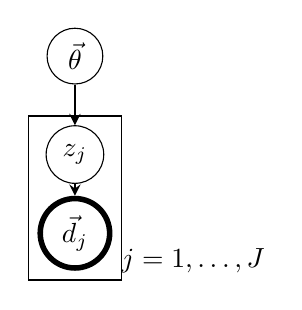
\begin{tikzpicture}[node distance=1cm]

\node (nz) [hyper] {$\vec{\theta}$};
\node (z) [param, below of=nz,yshift=-0.25cm] {$z_{j}$};
\node (mags) [data, below of=z] {$\vec{d}_{j}$};
\node (survey) [draw=black,fit={(mags.west)(z.north)(mags.south)(mags.east)}] {};
\node [xshift=1.5cm,yshift=0.25cm] at (survey.south) {$j=1,\dots,J$};

\draw [arrow] (nz) -- (z);
\draw [arrow] (z) -- (mags);

\end{tikzpicture}
\caption{This directed acyclic graph illustrates a hierarchical model.}
\end{center}
\end{figure}

For the purposes of this derivation, we assume the data for the entire survey $\{\vec{d}_{j}\}_{J}$ are independent measurements of $J$ data points $\vec{d}_{j}$, where $J$ itself is a Poisson random variable with expected value $J_{0}$.  However, this assumption that $z_{j}$ is independent of $z_{j'}$ must be false because of the shared physical processes governing observations of galaxies $j\neq j'$, such as the instruments with which they were observed and the covariances of $N(z)$.  Nonetheless, this assumption must be made in order to make the problem tractable.  Thus the likelihood of observing this data given a model $\vec{\theta}$ is said to be a set of independent samples $p(\vec{d}_{j}|\vec{\theta})$ with a shared $\vec{\theta}$ and can be expressed as Eq. \ref{eq:indie}.  \citep{for14}  It is important to note that $\int N(z)\ dz$ is not constrained to equal $J_{0}$ for the arbitrary proposed parameters $\vec{\theta}$.  It is also relevant to note that if we were to consider parameters $\vec{\theta}'$ describing $p(z)$ as defined in Eq. \ref{eq:params}, the log of the Poisson term will approach unity instead of $J_{0}$ for good choices of parameters.

\begin{eqnarray}
\label{eq:indie}
p(\{\vec{d}_{j}\}_{J}|\vec{\theta}) &=& e^{-\int N(z)\ dz}\prod_{j=1}^{J}p(\vec{d}_{j}|\vec{\theta})
\end{eqnarray}

We may apply Bayes' Rule, as in Eq. \ref{eq:bayes} to find the posterior probability of the hyperparameters $p(\vec{\theta}|\{\vec{d}_{j}\}_{J})$ from the likelihoods of Eq. \ref{eq:indie}.  Combining Eq. \ref{eq:indie} with Eq. \ref{eq:bayes} yields Eq. \ref{eq:posterior}.  We can further expand Eq. \ref{eq:posterior} into Eq. \ref{eq:marginalize} by involving the redshifts as parameters.

\begin{eqnarray}
\label{eq:bayes}
p(\vec{\theta}|\{\vec{d}_{j}\}_{J}) &=& \frac{p(\vec{\theta})}{p(\{\vec{d}_{j}\}_{J})}p(\{\vec{d}_{j}\}_{J}|\theta)
\end{eqnarray}

\begin{eqnarray}
\label{eq:posterior}
p(\vec{\theta}|\{\vec{d}_{j}\}_{J}) &=& \frac{p(\vec{\theta})}{p(\{\vec{d}_{j}\}_{J})}e^{-\int N(z)\ dz}\prod_{j=1}^{J}p(\vec{d}_{j}|\vec{\theta})
\end{eqnarray}

\begin{eqnarray}
\label{eq:marginalize}
p(\vec{\theta}|\{\vec{d}_{j}\}_{J}) &=& \frac{p(\vec{\theta})}{p(\{\vec{d}_{j}\}_{J})}e^{-\int N(z)\ dz}\prod_{j=1}^{J}\int\ p(\vec{d}_{j}|z_{j})\ p(z_{j}|\vec{\theta})\ dz_{j}
\end{eqnarray}

However, Eq. \ref{eq:marginalize} contains likelihoods $p(\vec{d}_{j}|z_{j})$ that in this case are inaccessible; it is worth discussing why this is the case.  Both empirical and data-driven methods for obtaining zPDFs effectively assign each set of photometry to both a redshift and some nuisance parameters $\vec{\alpha}$ related to the unobserved spectrum of the galaxy.  If we were to attempt to calculate likelihoods $p(\vec{d}_{j}|z_{j},\vec{\alpha}_{j})$, we would be unable to integrate out these nuisance parameters.  However, posteriors $p(z_{j},\vec{\alpha}_{j}|\vec{d}_{j})$ could be transformed to zPDFs $p(z_{j}|\vec{d}_{j})$ by integrating $p(z_{j},\vec{\alpha}_{j}|\vec{d}_{j})\ p(\vec{\alpha}$ with respect to $\vec{\alpha}$, given the prior distribution $p(\vec{\alpha})$ of those parameters.  Instead, we would like to work with posteriors rather than likelihoods in Eq. \ref{eq:marginalize}.  The method outlined here is valid regardless of how $p(z_{j}|\vec{d}_{j})$ is calculated, so the production of individual zPDFs is outside the scope of this paper; various methods have been presented by \citet{she11}, \citet{bal08}, \citet{car13}, and \citet{car14}.

To perform the necessary transformation from likelihoods to posteriors, we follow the reasoning of \citet{mar15}.  Let us consider the probability of the parameters $z_{j}$ conditioned on the data and an interim prior value of the hyperparameters $\vec{\theta}_{0}$ and rewrite Eq. \ref{eq:marginalize} as Eq. \ref{eq:trick}.  (While we would like any interim prior to be uninformative, this is rarely achievable, so we must be sure to integrate it out to avoid biasing our conclusions by this choice.)  We may then expand the denominator according to Eq. \ref{eq:bayes} to get Eq. \ref{eq:expand}.  The likelihood terms cancel as $p(\vec{d}_{j}|z_{j},\vec{\theta}_{0})=p(\vec{d}_{j}|z_{j})\ p(\vec{d}_{j}|\vec{\theta}_{0})$, yielding Eq. \ref{eq:cancel}.

\begin{eqnarray}
\label{eq:trick}
p(\vec{\theta}|\{\vec{d}_{j}\}_{J}) &=& \frac{p(\vec{\theta})}{p(\{\vec{d}_{j}\}_{J})}e^{-\int N(z)\ dz}\prod_{j=1}^{J}\int\ p(\vec{d}_{j}|z_{j})\ p(z_{j}|\vec{\theta})\ \frac{p(z_{j}|\vec{d}_{j},\vec{\theta}_{0})}{p(z_{j}|\vec{d}_{j},\vec{\theta}_{0})}\ dz_{j}
\end{eqnarray}

\begin{eqnarray}
\label{eq:expand}
p(\vec{\theta}|\{\vec{d}_{j}\}_{J}) &=& \frac{p(\vec{\theta})}{p(\{\vec{d}_{j}\}_{J})}e^{-\int N(z)\ dz}\prod_{j=1}^{J}\int\ p(\vec{d}_{j}|z_{j})\ p(z_{j}|\vec{\theta})\ p(z_{j}|\vec{d}_{j},\vec{\theta}_{0})\ \frac{p(\vec{d}_{j}|\vec{\theta}_{0})}{p(\vec{d}_{j}|z_{j},\vec{\theta}_{0})\ p(z_{j}|\vec{\theta}_{0})}\ dz_{j}
\end{eqnarray}

\begin{eqnarray}
\label{eq:cancel}
p(\vec{\theta}|\{\vec{d}_{j}\}_{J}) &=& \frac{p(\vec{\theta})}{p(\{\vec{d}_{j}\}_{J})}e^{-\int N(z)\ dz}\prod_{j=1}^{J}\ \int\ p(z_{j}|\vec{d}_{j},\vec{\theta}_{0})\ \frac{p(z_{j}|\vec{\theta})}{p(z_{j}|\vec{\theta}_{0})}\ dz_{j}
\end{eqnarray}

The argument of the integral in the posterior of Eq. \ref{eq:cancel} depends solely on knowable quantities and can be calculated for a given set of posteriors and the assumed prior upon which their determination was based.  We will have to assume a hyperprior $p(\vec{\theta})$ for the hyperparameters.  Since we cannot know $p(\{\vec{d}_{j}\}_{J})$, we sample the desired distribution $p(\vec{\theta}|\{\vec{d}_{j}\}_{J})$ using Monte Carlo-Markov chain (MCMC) methods.  

\section{Mock Data}
\label{sec:mock}

To enable direct comparison with previous results, we consider the $K=35$ redshift bins $B_{k}=[z^{B}_{k-1},z^{B}_{k}]$ over a range from $z_{0}=0$ to $z_{35}=1.1$ for which \citet{she11} calculated posteriors for the redshift of each galaxy based on observations of the apparent magnitude in the five photmetric filters of SDSS.  We shall take $\vec{\theta}$ to be a discretized parametrization of $N(z)$, where $\exp[\theta_{k}]$ is the average value of $N(z)$ over the redshift range of bin $B_{k}$.   Thus the expected number $J_{k}$ of galaxies in each bin is $\exp[\theta_{k}]\Delta_{k}$, where $\Delta_{k}\equiv z_{k}-z_{k-1}$, transforming Eq. \ref{eq:params} into Eq. \ref{eq:dparams}.

\begin{eqnarray}
\label{eq:dparams}
p(B_{k}|\vec{\theta}) &\equiv& \frac{J_{k}}{J} = \frac{\exp[\theta_{k}]\Delta_{k}}{J}
%N(B_{k}) &=& \theta_{k} = J\tilde{\theta}_{k}\Delta_{k}% \frac{\mathcal{N}_{k}}{\sum_{k=1}^{K}\mathcal{N}_{k}}
\end{eqnarray}

In order to simulate data, we select set a true, physically motivated redshift probability distribution $p^{0}(z|\vec{\theta})$, where $p(z|\vec{\theta})$ corresponds to $\vec{\theta}$ for $J=1$.  The convolution of a linear function and a sum of Gaussians is quite general and accurately generates features observed in the true $N(z)$.  The instance of $p^{0}(z)$ here is shown in Eq. \ref{eq:truepz}, where the constant $C_{c}$ indicates the relative amplitude of the Gaussian component centered at $z_{c}$ with variance $\sigma_{c}^{2}$.  The linear function is evaluated at the centers of the bins $\bar{z}_{k}=(z_{k+1}-z_{k})/2$ and is included to ensure that $\lim_{z\to0}N(z)=0$.  The construction of this probability density is illustrated in Fig. \ref{fig:truepz}.  

\begin{eqnarray}
\label{eq:truepz}
p^{0}(z_{k}) &=& \sum_{c=1}^{6}\bar{z}_{k}C_{c}\int_{z_{k}}^{z_{k+1}} \mathcal{N}(z_{c},\sigma^{2}_{c})dz
\end{eqnarray}

\begin{figure}
\label{fig:truepz}
\includegraphics[scale=0.5]{truePz.png}
\caption{We construct $p^{0}$ as a sum of Gaussians.}
\end{figure}

Up until this point, $\vec{\theta}^{0}$ has not been specified, nor have the individual zPDFs $p(z_{j}|\vec{d}_{j})$ been generated.  App. \ref{app:valid} presents several test choices of these quantities and demonstrates the method's validity in those intermediate test cases.  In the realistic case, we evaluate $p^{0}(z)$ over each bin to obtain $\vec{\theta}^{0}$ according to Eq. \ref{eq:truenz}, whose construction is illustrated in Fig. \ref{fig:truepz}.  

\begin{eqnarray}
\label{eq:truenz}
\theta_{k}^{0} &\equiv& \ln\left[J\int_{z_{k}}^{z_{k+1}}p^{0}(z) dz\right]
\end{eqnarray}

We next generate galaxy redshift likelihood functions as follows.  We first determine the number of galaxies $J$ in the survey by taking a Poisson sample around $J_{0}=1,000$.  We then assign a bin number $b_{j}=k$ from $k=1,\dots,K$ to each galaxy $j$ by randomly sampling the $K$ bins with weights given by the true redshift function as $\int_{z_{k}}^{z_{k+1}}p^{0}(z)dz$.  %Examples of some such samples for a fixed $J=1,000$ are shown in Fig. \ref{fig:obsnz}.

%\begin{figure}
%\label{fig:obsnz}
%\includegraphics[scale=0.5]{obsNz.png}
%\caption{Samples of the number of galaxies in each bin are generated as Poisson draws.}
%\end{figure}

We then assign each galaxy a true redshift $z_{j}$ chosen uniformly from within the bin $B_{b_{j}}$ to which it was assigned.  The true redshift of each galaxy is shifted by a random error according to Eq. \ref{eq:zshift} to simulate inaccuracy in measurements, yielding a shifted redshift $z_{j}'$ for each galaxy.  %Fig. \ref{fig:samples} shows histograms of the mock data generated.  It is worth noting that any method aiming to calculate the posterior should be unable to do better than the ``observed redshifts'' that go into generating the data.  SOMEHOW THIS IS NOT TRUE FOR THIS DATA, BUT HOW?

\begin{mathletters}
\begin{eqnarray}
\label{eq:zshift}
z_{j}' &=& z_{j}+e_{j}\\
p(e_{j}) &=& \mathcal{N}(0,\delta_{j})\nonumber\\
\delta_{j} &=& \frac{\sum_{b_{k}=1}^{K}(z_{b_{k}}-z_{b_{k}-1)}}{K}(1+z_{j})\nonumber
\end{eqnarray}
\end{mathletters}

%\begin{figure}
%\label{fig:samples}
%\includegraphics[scale=0.5]{exdata.png}
%\caption{The true $\vec{\theta}$ chosen for this test is plotted here, along with histograms of the true redshifts sampled from it and the shifted redshifts resulting from the mock data generation procedure.}
%\end{figure}

The discretized posterior $p(B_{k}|\vec{d}_{j})$ for each galaxy is taken to be Gaussian with a mean equal to the shifted redshift and a standard deviation proportional to $1+z_{j}$ to simulate the fact that uncertainty increases with redshift.  According to the above, "the data" are thus comprised of $J$ pairs $(z_{j}',\delta_{j})$.  The observed probability that galaxy $j$ has a redshift in bin $k$ is given by Eq. \ref{eq:zdist}.  As a final step, all posteriors are normalized such that they integrate to unity over the redshift range spanned by the bins.  Fig. \ref{fig:pzs} shows a few examples of simulated posteriors.

\begin{eqnarray}
\label{eq:zdist}
p(B_{k}|\vec{d_{j}}) = \int_{z_{k}}^{z_{k+1}} \frac{1}{\sqrt{2\pi\delta_{j}^{2}}}\exp\left[-\frac{(z_{j}'-z)^{2}}{2\delta_{j}^{2}}\right]\ dz
\end{eqnarray}

\begin{figure}
\label{fig:pzs}
\includegraphics[scale=0.5]{lik-samps.png}
\caption{Several random redshift likelihood functions selected from the $p^{0}(z)$ of Fig. \ref{fig:truepz} are shown here.  Note that the width of the Gaussian increases with redshift according to Eq. \ref{eq:zdist}.}
\end{figure}

The posterior for the entire dataset introduced in Eq. \ref{eq:cancel} may be re-expressed as Eq. \ref{eq:fullpost} in terms of the $K$ bins.  It is valuable to verify that the posterior is maximized for the true $N(z)$ that generated a particular set of simulated data.

\begin{eqnarray}
\label{eq:fullpost}
p(\vec{\theta}|\{\vec{d}_{j}\}_{J}) &=& \frac{p(\vec{\theta})}{p(\{\vec{d}_{j}\}_{J})}\ \exp\left[-\sum_{k=1}^{K}\exp[\theta_{k}]\Delta_{k}\right]\ \prod_{j=1}^{J}\ \sum_{k=1}^{K}\ p(B_{k}|\vec{d}_{j})\ \frac{\exp[\theta_{k}]}{\exp[\theta_{k}^{0}]}\Delta_{k}
\end{eqnarray}

\section{Application}
\label{sec:app}

The Metropolis-Hastings algorithm is applied to sample the posterior of Eq. \ref{eq:fullpost}.  We work with log probabilities from this point forward for computational efficiency and numerical stability.  Since $p(\{\vec{d}_{j}\}_{J})$ is in general unknown, we will also commence working with $\tilde{p}(\vec{\theta}|\{\vec{d}_{j}\}_{J})$, a quantity proportional to Eq. \ref{eq:fullpost}, which shall be called the "pseudo-posterior," the log of which is given in Eq. \ref{eq:logpost}.

\begin{eqnarray}
\label{eq:logpost}
\ln[\tilde{p}(\vec{\theta}|\{\vec{d}_{j}\}_{J})] &=& \ln[p(\vec{\theta})]-\exp[\vec{\theta}]\cdot\vec{\Delta}+\sum_{j=1}^{J}\ \ln\left[\sum_{k=1}^{K}\ \exp\left[\ln[p(B_{k}|\vec{d}_{j})]+\theta_{k}-\theta_{k}^{0}+\ln[\Delta_{k}]\right]\right]
\end{eqnarray}

The procedure is initialized with an interim prior equal to a multivariate normal distribution with mean and covariance given by Eq. \ref{eq:covmat}.  The mean chosen here is that of a flat distribution.  The constants $q$, $a$, and $e$ are small numbers chosen to permit draws from the distribution in question to reproduce shapes similar to that of the true $N(z)$ set in Sec. \ref{sec:mock}.

\begin{eqnarray}
\label{eq:covmat}
\theta^{0}_{k} &=& \ln[J_{0}]-\ln[K]-\ln[\Delta_{k}]\\
\Sigma_{kk'} &=& q\exp^{-\frac{a(k-k')^{2}}{2}}+e\cdot\mathbb{I}
\end{eqnarray}

At each iteration $i$, a proposal distribution $\vec{\theta}^{i}$ generated from the prior distribution shown in Eq. \ref{eq:covmat}.  %Some examples of samples from the initialization value are shown in Fig. \ref{fig:priors}.

%\begin{figure}
%\label{fig:priors}
%\includegraphics[scale=0.5]{samples5.png}
%\caption{Several random samples of $\vec{\theta}$ from the distribution of Eq. \ref{eq:covmat} are shown here.  %As $a$ increases, more peaks are permitted and the distribution becomes less smooth.  For a set value of $q$, the amplitude of deviations from the mean decreases with $a$.
%}
%\end{figure}

The algorithm is outlined below.

\begin{enumerate}
\item \label{it:randsamp} Randomly sample Eq. \ref{eq:covmat} to generate a proposal $\vec{\theta}'$.
\item Calculate the log pseudo-posterior as in Eq. \ref{eq:logpost} to produce $\ln\tilde{p}(\vec{\theta}'|\{vec{d}_{j}\}_{J})$.
\item Calculate $r=\ln\tilde{p}(\vec{\theta}'|\{vec{d}_{j}\}_{J})-\ln\tilde{p}(\vec{\theta}|\{vec{d}_{j}\}_{J})$.
\item If $r\geq0$, set and record $\vec{\theta}=\vec{\theta}'$.\\
If $r<0$, select a random number $n$ from the uniform distribution between 0 and 1.
\begin{enumerate}
\item If $n<\exp[r]$, record $\vec{\theta}_{r+1}=\vec{\theta}'$ and set $\vec{\theta}=\vec{\theta}'$
\end{enumerate}
\item Check if the threshold has been achieved; if not, return to Step \ref{it:randsamp}.
\end{enumerate}

Here, the threshold was $I=10^{4}$ iterations.  All accepted proposals from one instance of the code are shown in Fig. %\ref{fig:results}
.  The acceptance fraction was $\sim0.1\%$ for this and other runs.  Since 10000 iterations likely doesn't even get through the ``burn-in'' period of the algorithm, this acceptance fraction is not surprising!  If I were convinced it were otherwise valid, I would run it until some convergence criterion were achieved.  However, since that might take quite some time, I will conservatively refrain from doing so.

%\begin{figure}
%\label{fig:results}
%\includegraphics[scale=0.75]{compare-results.png}
%\caption{Accepted proposal values of $\vec{\mathcal{N}}$ are shown here, along with the true value in black.}
%\end{figure}

\section{Discussion}

It is desirable to compare this result to what would have been obtained by the method of \citet{she11}, which directly calculates the posterior for the entire dataset using the posteriors for each galaxy according to Eq. \ref{eq:sheldon}.

\begin{eqnarray}
\label{eq:sheldon}
p(B_{k}) &=& \sum_{r=1}^{R}p_{r}(B_{k}|\vec{d}_{j})
\end{eqnarray}

To do this, I calculate the posteriors $p(z|\vec{d}_{j})$ for each galaxy using Eq. \ref{eq:posts}, the product of the estimate of $\vec{\theta}$ and the likelihood for each galaxy.  This is done for all accepted values of $\vec{\theta}$.

\begin{eqnarray}
\label{eq:posts}
p_{r}(B_{k}|\vec{d}_{j}) &=& p(\vec{d}_{j}|B_{k})p(\vec{\theta}^{r}|\textul{D})
\end{eqnarray}

%Fig. \ref{fig:sheldon} compares the result of summing the posteriors as in Eq. \ref{eq:sheldon} with the result of the MCMC solutions of Eq. \ref{eq:bayes}.  The method of \citet{she11} underestimates the probability of observing low redshifts.  As one would expect, the MCMC estimate irreversibly loses some substructure because of the shifting error added to the simulated data.

%\begin{figure}
%\label{fig:sheldon}
%\includegraphics[scale=0.5]{compare-sheldon.png}
%\caption{The result of applying Eq. \ref{eq:sheldon} is shown in red, the average accepted posterior sample from the method presented here is shown in blue, and $p(z)$ for the observable redshifts of Eq. \ref{eq:zshift} is shown in black.  The sum of squared differences between the result of each method and the true value are also shown; one can see that the \citet{she11} approach has larger errors.}
%\end{figure}

%\acknowledgments

\appendix{}
\label{app:test}

The method herein developed was rigorously tested to ensure its validity.  A few mock catalogs were generated to simulate specific test cases to validate the code, and the results of the tests were evauated on the basis of four diagnostics

\section{Diagnostics}
\label{app:diag}

Before reporting on the validation tests, it is first necessary to define the diagnostic measures used to evaluate the results of the test.  See \citet{for12} for a more complete exploration of these metrics.

\subsection{Autocorrelation Time}
\label{app:acorr}

The autocorrelation time is effectively a measure of the convergence rate of the method and can be described as the expected number of iterations necessary to accept a sample independent of the current sample.  A sampler that converges faster will have a smaller autocorrelation time, and smaller autocorrelation times are preferable because it means fewer iterations are wasted on non-independent samples when independent samples are desired.  Typically, the autocorrelation time decreases with successive iterations through a burn-in phase before leveling out.

\subsection{Acceptance Fraction}
\label{app:afrac}

Though there is no hard rule for the optimal acceptance fraction for a sampler, we would like it to be high enough that we accept a fair number of samples but low enough that the samples do approach a single distribution.  Commonly accepted goals tend to be between 0.2 and 0.5.  Typically, the acceptance fraction is high during the burn-in phase until some independence from the initial values is achieved, after which it levels out.

\subsection{Probability Evolution}
\label{app:probs}

In order to evaluate the extent of the burn-in phase, it can be helpful to examine the evolution of the posterior probability of each accepted set of parameters.  Though the probability associated with the initial values will likely be quite low, the probability should improve for subsequent accepted parameter values.  As with the diagnostics of Secs. \ref{app:afrac} and \ref{app:probs}, the posterior probability of samples will asymptotically approach some more favorable value with more iterations.  The burn-in phase may be identified as the number of iterations necessary before the probabilities are sufficiently close to the value at which they level out.  Samples accepted during the burn-in phase are typically discounted from analysis.

\subsection{Parameter Evolution}
\label{app:params}

A final diagnostic used here is the evolution of the parameter values themselves.  We would like to see each walker move throughout parameter space rather than remaining stationary or in some small region corresponding to some local maximum of probability.  We can visually inspect the parameter values each walker takes over successive iterations to ensure that the walkers are not being caught in small regions of parameter space.

\section{Validation}
\label{app:valid}

Here we report on the results of simple, unrealistic tests after outlining their goals and setups, including the mock data used in each.

\subsection{}
\label{app:fake}

We first test the accuracy of the sampler in a simplified case with a delta function for the true $N(z)$.  The parameters $\vec{\theta}^{0}$ defining the true redshift distribution will thus take the form of Eq. \ref{eq:faketheta}.  Here we use the full set of $K=35$ redshift bins described in Sec. \ref{sec:mock} and set the true bin number $k_{0}$ as the bin where the distribution defined by the weights from \ref{fig:truepz} is maximized.

\begin{eqnarray}
\label{eq:faketheta}
\exp[\theta_{k}^{0}] &=& \left\{\begin{array}{cc}0&k\neq k_{0}\\J/\Delta_{k}&k=k_{0}\end{array}\right\}
\end{eqnarray}

The mock data consists of a set number $J=J_{0}$ galaxies with a single true redshift $z^{s}$ equal to the midpoint $\bar{z}_{k_{0}}$ of bin $k_{0}$.  The individual galaxy posteriors are taken to be single Gaussians with a standard deviation equal to $\bar{\Delta}(1+z^{s})$ centered at an observed redshift $z^{p}_{j}$ according to Eq. \ref{eq:zdist}.  The observed redshift $z^{p}_{j}$ is itself a draw from a Gaussian with a standard deviation of $\bar{\Delta}(1+z^{s})$ centered at $z^{s}$ according to Eq. \ref{eq:zshift}.  Survey sizes of $J_{0}=2,200$ are considered for this test.

We choose a prior of a multivariate normal centered at a flat $\vec{\theta}^{0}$ with the identity as the covariance matrix, as in Eq. \ref{eq:fakeprior}.  Examples of draws from this prior are shown in Fig. \ref{fig:fakeprior}.  We test three procedures for generating initial values for the walkers: samples taken from the prior distribution, samples taken as a Gaussian ball around the mean of the prior distribution, and samples taken as a Gaussian ball around a single sample from the prior distribution.  The sampler is run with 70 walkers initialized as shown in Fig. \ref{fig:fakeival}.

\begin{eqnarray}
\label{eq:fakeprior}
p(\vec{\theta}) &=& \int_{z_{k}}^{z_{k+1}}\frac{1}{\sqrt{2\pi}}\exp[-\frac{1}{2}(\vec{\theta}^{0}-\vec{\theta})^{T}\textul{I}(\vec{\theta}^{0}-\vec{\theta})]dz
\end{eqnarray}

\begin{figure}
\label{fig:fakeprior}
\includegraphics[scale=0.25]{priorsamps.png}
\caption{Examples of draws from the prior of Eq. \ref{eq:fakeprior}.}
\end{figure}

\begin{figure}
\label{fig:fakeival}
\includegraphics[scale=0.25]{initializations.png}
\caption{Three different methods are tested for selecting the initial values.}
\end{figure}

This test indicates the sampler is working as expected.

\begin{figure}
\label{fig:dumbestacor}
\includegraphics[scale=0.25]{acorr.pdf}
\caption{The autocorrelation times are very low, indicating extremely fast convergence of the sampler.}
\end{figure}

\begin{figure}
\label{fig:dumbestfrac}
\includegraphics[scale=0.25]{fracs.pdf}
\caption{The acceptance fractions are a bit low but not far from the desired range for all initialization procedures.  As expected, the acceptance fraction is lower in general for larger numbers of data points, as the parameters must be chosen to fit a more complicated likelihood.}
\end{figure}

\begin{figure}
\label{fig:dumbestprob}
\includegraphics[scale=0.25]{lnprobs.pdf}
\caption{This plot shows the log probabilities of walkers as a function of iteration number.  One can see the duration of the burn-in period.}
\end{figure}

\begin{figure}
\label{fig:dumbestparam}
\includegraphics[scale=0.25]{results.pdf}
\caption{The results of the simulation may be seen here.  By way of the $\chi^{2}$ statistic (incorrectly labeled $\sigma^{2}$ in this draft), one can see that in estimating the log of $N(z)$, the result of the method of \citet{she11} is inferior to the method presented in this paper.}
\end{figure}

%\subsubsection{}
%\label{app:dumber}

%We next consider a set of $J$ galaxies representing a draw from the Poisson distribution $P(J_{0},J_{0})$ for $J_{0}=100$.  The galaxies share a single true redshift $z^{s}$ arbitrarily chosen to be the midpoint of the redshift bin with the largest $\theta_{k}$.  The redshift posteriors are taken to be single Gaussians centered at observed redshifts $z^{p}_{j}\sim N(z^{s},\bar{\Delta}(1+z^{s}))$ with shared variances of $\bar{\Delta}(1+z^{s})$. 

%\subsubsection{}
%\label{app:dumb}

%The last test case is comprised of a set of $J$ galaxies representing a draw from the Poisson distribution $P(J_{0},J_{0})$ for $J_{0}=1000$.  The true galaxy redshift bins $b_{j}=k$ from $k=1,\dots,K$ are assigned to each galaxy $j$ by randomly sampling the $K$ bins with weights given by the true redshift function of Eq. \ref{eq:truenz} as $\int_{z_{k}}^{z_{k+1}}p^{0}(z)dz$. True redshifts $z^{s}_{j}$ are assigned within these bins assuming a random uniform distribution within each bin.  The redshift posteriors are taken to be single Gaussians centered at observed redshifts $z^{p}_{j}\sim N(z^{s}_{j},\bar{\Delta}(1+z^{s}_{j}))$ with variances $\sigma_{j}\sim N(z^{s}_{j},\bar{\Delta}(1+z^{s}_{j}))$. 

\subsection{}

\subsection{}

\bibliography{references}

\end{document}

\end{thebibliography}